\begin{problem}%
{Космические исследования}%
{\textsl{стандартный ввод}}%
{\textsl{стандартный вывод}}%
{1 секунда}%
{64 мегабайта}{}

Отделу космических исследований поступило задание сфотографировать из космоса $n$ объектов в заданной области. Область имеет форму квадрата размером $50 \times 50$ километров. Если разделить ее на квадраты размером $1 \times 1$ километр, то интересующие отдел объекты окажутся в центрах некоторых единичных квадратов.\\

Введем систему координат, направив ось OX с запада на восток и ось OY с юга на север. Тогда каждому единичному квадрату будут сопоставлены координаты в диапазоне от 1 до 50, как показано на рисунке ниже.

\begin{center}
    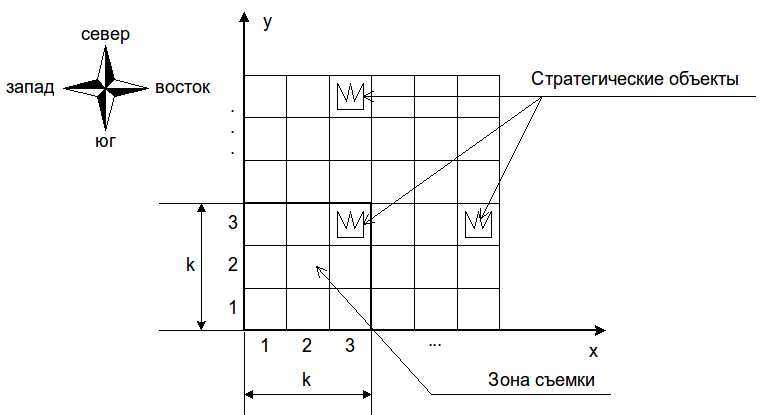
\includegraphics[scale=0.5]{images/2.png}
\end{center}

Для космической съемки используется специальный фотоаппарат высокого разрешения, установленный на космическом спутнике. Фотоаппарат может делать снимки квадратных участков земной поверхности размером $k \times k$  километров. Исходно аппарат наведен на юго-западный угол заданной области, то есть, если сделать снимок, на нем будут видны единичные квадраты с координатами $x$ и $y$ от 1 до $k$ километров.\\

С помощью специальных двигателей можно изменять орбиту спутника, что приводит к изменению участка съемки. За один день орбиту спутника можно изменить таким образом, что участок съемки сместится либо на один километр на запад, либо на один километр на восток, либо на один километр на север. Переместить участок съемки на юг невозможно. Непосредственно между перемещениями спутника можно сделать снимок, временем съемки можно пренебречь.\\

Руководство отдела заинтересовалось вопросом: за какое минимальное количество дней можно сделать снимки всех объектов заданной области.\\

Требуется написать программу, которая по заданному расположению объектов и размеру снимка $k$ определит минимальное время, за которое можно сделать снимки всех объектов заданной области.

\InputFile

Первая строка входного файла содержит два целых числа: $n$ и $k$ ($1 \le n \le 1000$, $1 \le k \le 5$).\\

Следующие $n$ строк содержат по два целых числа: $x_i$ и $y_i$ — координаты объектов в заданной области ($1 \le x_i, y_i \le 50$).

\OutputFile

В выходном файле должно содержаться одно целое число: минимальное количество дней, которое требуется для получения снимков всех объектов в заданной области.

\Examples

\begin{example}
\exmp{
4 1
1 1
10 2
1 3
10 4
}{%
30
}%
\exmp{
4 2
1 1
10 2
1 3
10 4
}{%
10
}%
\exmp{
1 1
1 1
}{%
0
}%
\exmp{
3 3
3 3
3 6
6 3
}{%
7
}%
\end{example}

\Explanations

В первом примере возможна следующая последовательность действий: сделать снимок, 9 раз сместиться на восток, сместиться на север, сделать снимок, 9 раз сместиться на запад, сместиться на север, сделать снимок, 9 раз сместиться на восток, сместиться на север, сделать снимок. Всего требуется 30 перемещений участка съемки.\\

Во втором примере объекты расположены там же, но размер снимка больше, поэтому можно действовать так: сделать снимок, сместиться на север, сделать снимок, 8 раз сместиться на восток, сделать снимок, сместиться на север, сделать снимок. Всего требуется лишь 10 перемещений участка съемки.\\

В третьем примере перемещать участок съемки не требуется, можно просто сделать снимок.\\

Четвертый пример соответствует приведенному выше рисунку.

\end{problem}